\documentclass[11pt, a4paper]{article}
\usepackage[margin=2cm]{geometry}
\usepackage{amsmath, amssymb}
\usepackage{graphicx}
\usepackage{float}
\usepackage{aligned-overset}

% partielle ableitungen
\newcommand{\delr}{\partial_r}
\newcommand{\deltheta}{\partial_\theta}
\newcommand{\delphi}{\partial_\varphi}

% elektrische feldkonstante
\newcommand{\epsz}{\epsilon_0}
% 1 / 4pi eps
\newcommand{\kco}{\frac{1}{4\pi\epsilon_0}}

% fancy header
\usepackage{fancyhdr}
\fancyhf{}
% vspaces in den headern fuer Distanzen notwendig
% linke Seite: Namen der Abgabegruppe
\lhead{\textbf{Benedikt Sander \\Tahir Kamcili \\ Matthias Maile}\vspace{1.5cm}}
% rechte Seite: Modul, Gruppe, Semester
\rhead{\textbf{Astroteilchenphysik\\Sommersemester 2020}\vspace{1.5cm}}
% Center: nr. des blattes
\chead{\vspace{2.5cm}\huge{\textbf{5. Übungsblatt}}}
% benoetigt damit der eigentliche Text nicht in der Überschrift steckt
\setlength{\headheight}{4cm}

% zum zeichnen tikz
\usepackage{tikz}

\begin{document}
\thispagestyle{fancy}
\noindent
{\large\textbf{Aufgabe 13}} \\[0.2cm]
a) Wenn wir uns den Bereich, den wir sehen in ``Ebenen`` aufteilen, so erhalten wir (bei richtigem 
Winkel) für jede Ebene einzeln betrachtet die Wahrscheinlichkeit
\[ P = \frac da. \]
Da allerdings die vorherigen Wahrscheinlichkeite rausgerechnet werden müssen lautet die 
Wahrschihenlichekeit, an der $n$-ten Ebene auf einen Baum zu treffen:
\[
	P(n) = \left(1 - \sum_{i = 1}^{n-1} P(i) \right) \frac da 
\]
Der Plot der Wahrscheinlichkeitsverteilung lässt dabei einen exponentiellen Zusammenhang vermuten, mit
einem ``Verlust`` von 0.05 pro Ebene:
\begin{figure}[H]
	\centering
	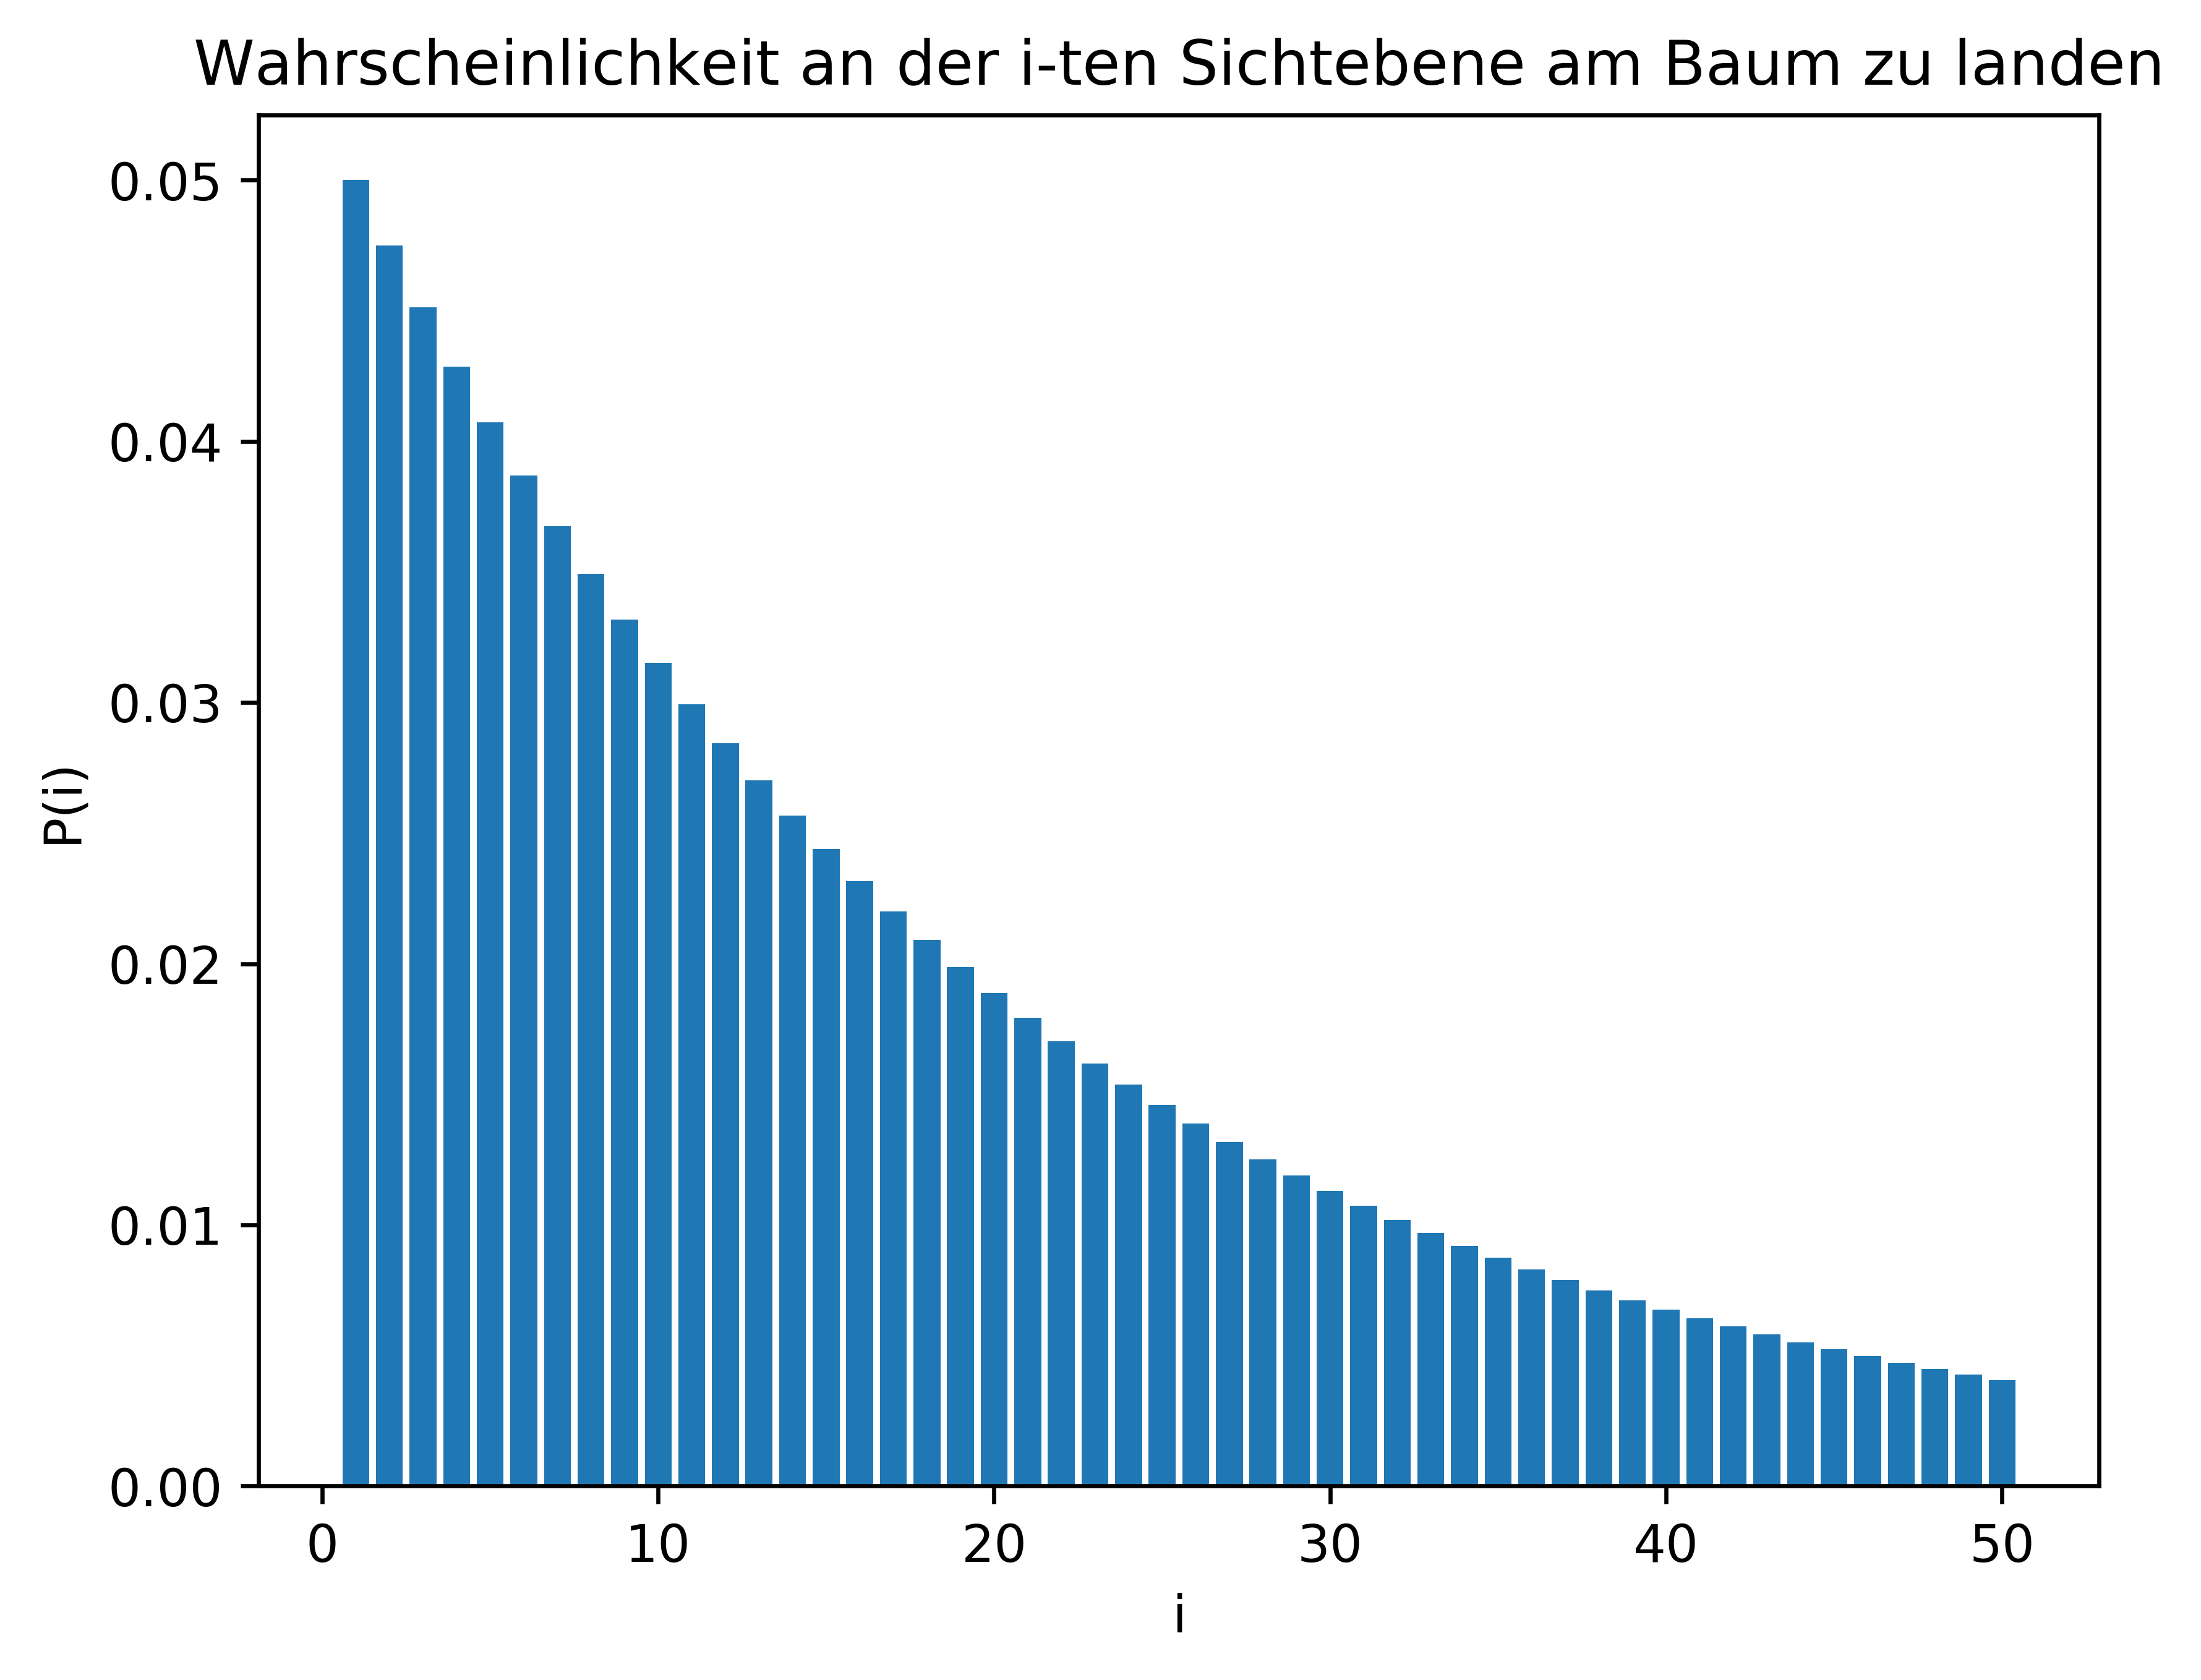
\includegraphics[width=10cm]{13.png}
\end{figure}
Mit dem Anfangswert $P(1) = \frac da = 0.05$ lautet die Wahrscheinlichkeitsfunktion:
\[
	P(i) = 0.05 \cdot \exp\left( \frac{0.95 \cdot i}{m}\right)
\]
Der Mittelwert lautet dann
\[
	\mu = \sum_{i=1}^\infty i \cdot P(i) \approx 20m
\]

\newpage
\setlength{\headheight}{0cm}

b)
Im dreidimensionalen können wir den Raum in Kugelschalen aufteilen, sodass, wenn wir als Dicke einer 
Kugelschale ein Parsc wählen die Wahrscheinlichkeit erhalten:
\[
	P = \frac{\text{Freie Fläche}}{\text{bedeckte Fläche}} = \frac{\rho \cdot V}{\pi r^2}
	=\frac{\rho \cdot \left(R^3 - r^3\right) \cdot R_\odot^2}{r^2}
\]
Mit der Schalendicke erhalten wir:
\begin{align*}
	P(r) 
	&= \frac{\rho \cdot \left( (r+ 1pc)^3 - r^3 \right) \cdot R_\odot^2}{r^2} \\
	&= \frac{\rho \cdot \left( r^2 \cdot pc + r \cdot pc^2 \right) \cdot R_\odot^2}{r^2} \\
	&= \frac{10^{-10} \cdot \left( \frac{r^2}{pc^2} + \frac{r}{pc} \right) \cdot R_\odot^2}{r^2} \\
	&= 10^{-10} \cdot \left( \frac{R_\odot^2}{pc^2} + \frac{R_\odot^2}{r \cdot pc} \right)
\end{align*}
Aufgrund des großen Abstandes zwischen den Sternen und der geringen Dichte wird die mittlere freie 
Weglänge eine sehr große Distanz sein.

\vspace{0.5cm}

c) Laut dem Ergebnis aus b) müsste der Nachthimmel hell sein. Das ist
offensichtlich nicht der Fall, mit mehreren Ursachen:
\begin{itemize}
	\item Sterne besitzen eine endliche Lebensdauer (es müssten als durchgehend so viele neu 
	entstehen wie verschwinden)
	\item Das Universum besitzt eine endliche Lebenszeit, d.h. dass das Licht von weit entfernten Galaxien 
	``noch nicht die Zeit hatte`` um zur Erde zu gelangen.
	Diese Distanz heißt Hubble-Radius und beträgt 
	\[ r_h = 14.2 \cdot 10^9 \text{ Lichtjahre} < \text{ Ergebnis aus b)}\]
	\item Aufgrund der kosmischen Rotverschiebung würde sichtbares Licht von weit entfernten 
	Sternen ins rote verschoben werden, sodass neben dem zweiten Punkt auch die Rotverschiebung ein 
	``Limit`` für die Sichtweite darstellt
	\end{itemize}

\end{document}
